\documentclass[5p, times]{elsarticle}

%%%%%%%%%%%%%%   Preample  %%%%%%%%%%%%%%%%%%
%% for comment (texts in between \begin{comment} and \end{comment} will be ignored)
\usepackage{comment} 

%% The amssymb package provides various useful mathematical symbols
\usepackage{amssymb}
%% The amsthm package provides extended theorem environments
\usepackage{amsthm}

%% for celcius symbol
\usepackage{textcomp}

%% for units
\usepackage{siunitx}

%% multirow
\usepackage{multirow}

%% The lineno packages adds line numbers. Start line numbering with
%% \begin{linenumbers},  end it with \end{linenumbers}. Or switch it on
%% for the whole article with \linenumbers.
%\usepackage{lineno}
%\linenumbers

%% package for subfigure environment
\usepackage{subcaption}

%% package for type Greek letters without entering into math-mode
\usepackage{textgreek}

%% package for large picture in two-colume
\usepackage{dblfloatfix}
%\usepackage{fixltx2e}

%% only jpg pdf eps are allowed, tiff format are not allowed in latex
%% eps in principle can't be compiled by pdflatex, pdf not compiled by latex, but Kile can do some intermedate conversion to allow this happen.
\DeclareGraphicsExtensions{.pdf, .eps, .jpg}
%%opening
\journal{NIMA}

\begin{document}

%%%%%%%%%%%%%% Front Matter %%%%%%%%%%%%%%%%%%
\begin{frontmatter}

\title{A versatile PMT test bench and its application in the PSD detector of DAMPE}
%%\title{Title with footnote\tnoteref{t1}}
%%\tnotetext[t1]{FootNote for title}

\author[imp, ucas, lzu]{Yong Zhou}
%\ead{yong@impcas.ac.cn}

\author[imp]{Yuhong Yu}
%%\ead{yuyuhong@impcas.ac.cn}

\author[imp]{Zhiyu Sun\corref{corresponding_author}}
\cortext[corresponding_author]{Corresponding author}
\ead{sunzhy@impcas.ac.cn}

%% Additional Author information %%
%%\author[ano]{Anonymous\fnref{fn1}}
%%\ead{anonymous@anonymous.cn}
%%\fntext[fn1]{FootNote for Anonymous author}

\address[imp]{Institute of Modern Physicas, Chinese Academy of Sciences,  509 Nanchang Road,  Lanzhou,  730000,  P.R.China}
\address[ucas]{Graduate University of the Chinese Academy of Sciences,  19A Yuquan Road,  Beijing,  100049,  P.R.China}
\address[lzu]{School of Nuclear Science and Technology,  Lanzhou University,  222 South Tianshui Road,  Lanzhou,  730000,  P.R.China}
%%\address[ano]{Anonymous Address of Anonymous author}

%%
\begin{abstract}
blablabla
\end{abstract}

%%
\begin{keyword}
keyword1
\sep keyword2
\sep keyword3

%% PACS codes here,  in the form: \PACS code \sep codes

%% MSC codes here,  in the form: \MSC code \sep code
%% or \MSC[2008] code \sep code (2000 is the default)

\end{keyword}

\end{frontmatter}

%%%%%%%%%%%%%%%%  Introduction  %%%%%%%%%%%%%%%%%%%%%%%
\section{Introduction}
\label{sec:introduction}

\begin{comment}
DArk Matter Paricle Explorer(DAMPE)~\cite{Chang_Jin_dampe} is a satellite-borne particle detector for dark matter search and cosmic ray study.
It is designed to cover the energy range from 5~GeV to 10~TeV for electrons and photons with an energy resolution of 1\% at 800~GeV, from 100~GeV to 1~PeV for heavy ions with an energy resolution better than 40\% at 800~GeV.

Plastic scintillator Strip Detector(PSD), which sits at the topmost of the satellite, is a key component of DAMPE detector.
By measuring the energy deposit of particles pentrating through it, PSD serves as a anti-coincidence detector for e/$\gamma$ discrimination as well as a detector for charge measurement up to Z=20.
PSD consists of 82 plastic scintillator strips(EJ-200~\cite{ej200}) of dimention $864mm\times28mm\times10mm$, each readout at both ends by a Hamamastu R4443-Mod2 photomultiplier tube.
These strips are arranged into two orthogonally oriented layers, convering an effective area of $820mm\times820mm$.
Each PMT is readout at both dynode 5 and dynode 8 with different gains to cover the large dynamic range from $\sim$0.5~MIPs to $\sim$700~MIPs.
The readout signals are processed by a highly-sensitive ASIC chip(VA32) with the range of 0-14~pC, and then digitized by an ADC with 14~bits resolution.

Unlike groud-based experiments, the power supply system of DAMPE payload can only provide discrete high voltage levels with an interval of 30~V.
Furthermore, every 6 or 7 PMTs of PSD form a HV-group and share the same high voltage channel.
In this case, the ususal method of fine-tuning individual PMT's high voltage to get optimal gain is not available.  
The characteristics of PMTs in the same HV-group should have similar dependency on voltage.
Thus a careful selection of the tubes is mandatory to get uniform energy response across the whole detector and optimal utilization of the mesuring range.
For this selection, the gain of dynode 5 and dynode 8 as a function of supplying voltage needs to be measured precisely.  

Considering the large number of tubes involved in the Selection phase and Qualification phase, a PMT test bench for bulk testing was designed and contructed to facilitate this work.
500 bare R4443-Mod2 tubes were thoroughly tested and 200 of them were selected for production and qualification.
Finally, 164 PMT modules with the optimal characteristics were installed.
While mainly developped for the DAMPE-PSD project, this test bench has been designed to be as versatile as possible and can be upgaded seamlessly for future experiments.
The detailed description of the test bench will be given in Sec.\ref{sec:description}.Some key characteristics of the test bench is summarized in Sec.\ref{sec:char_testbench}.
The testing results of PSD PMTs and the corresponding selection procedure will be discussed in Sec.\ref{sec:pmt_test}.
\end{comment}

%%Photomultiplier tubes(PMTs) are widely used as photosensors in various fields, such as particle detectors in experimental physics and medical equipments in medical diagnosis.
%%PMT features in high sensitivity, large gain and easy-operation, whic make it still popular about 80 years after its invention.
Photomultiplier tubes(PMTs), due to its high gain,large dynamic range and easy-operation, are widely used as photosensors in particle detectors.
Large detectors usually contain hundreds, even thousands of PMTs as detection channels.
As the characteristics of PMTs exhibit large individual differences, a
However, 
In this case, a test of all PMTs before assembly is mandatory for the following reasons:
\begin{enumerate}
 \item Parameters from manufacturers are usually tested using tungstun filament lamp and only give a general and rough estimation of the performance of tubes.
 They are not suitable for accurate tuning of tubes in  where the light intensity is much lesser.
 \item Characteristics of PMTs ususally exhibit large individual differences.
 Only PMTs 
 \item The gain of PMT is dependent on supplying voltage.especially the gain.
 To get a uniform response across the whole system and better resolution, a tuning of the position and supplying voltage a thorough characterization of each PMT is needed.
 \item Furthermore, some of the parameters may not provided by 
 \item As a qualification step, the performance of all PMTs needs to be verified.
 PMTs which failed the specification should be rejected.
\end{enumerate}


The major design considerations of the test bench are summarized as follows:
\begin{itemize}
 \item \textit{Large capacity}: This is the primary driving force for developping the test bench as indicated in Sec.\ref{sec:introduction}.
 Testing multiple PMTs simultaneously can increase the efficiency and save project time tremendously. 
 \item \textit{Automation}: A single test run ususally takes several hours,  during which most operations are trivial jobs like change voltage value, change light intensity, start/stop DAQ, and so on.
 Manual operations are sometimes unreliable in such a long time testing period.
 Thus computer controllable hardwares should be used wherever possible and corresponding software should be developped to automate these trivial operations.
 Manual intervention is only needed in the beginning when mounting PMTs and configuring the software and in the end when unmounting PMTs and assessing testing result. 
 \item \textit{Versatility}: The test bench is not designed for single use.
 After its initial use in DAMPE PSD, it will be used for other experiments with different testing requirements.
 T\-h\-u\-s potential use cases should be considered and appropriate hardwares should be set up in the first place.
 %In particular, positon scanning capability is desirable for characterization of large area PMTs. 
 \item \textit{Flexibility}: As a by product of versatiltiy, flexibility is needed both in terms of hardware and software.
 The hardware platform should be extensible and allow complex testing configurations.
 The software should accommodate any changes in the hardware easily, while keeping the high level functionality unchanged and portable. 
\end{itemize}

%%%%%%%%%%%%%%%% Main Text Body %%%%%%%%%%%%%%%%%%%%%%%
\section{Description of the test bench}
\label{sec:description}

\begin{figure*}[t]
 \centering
 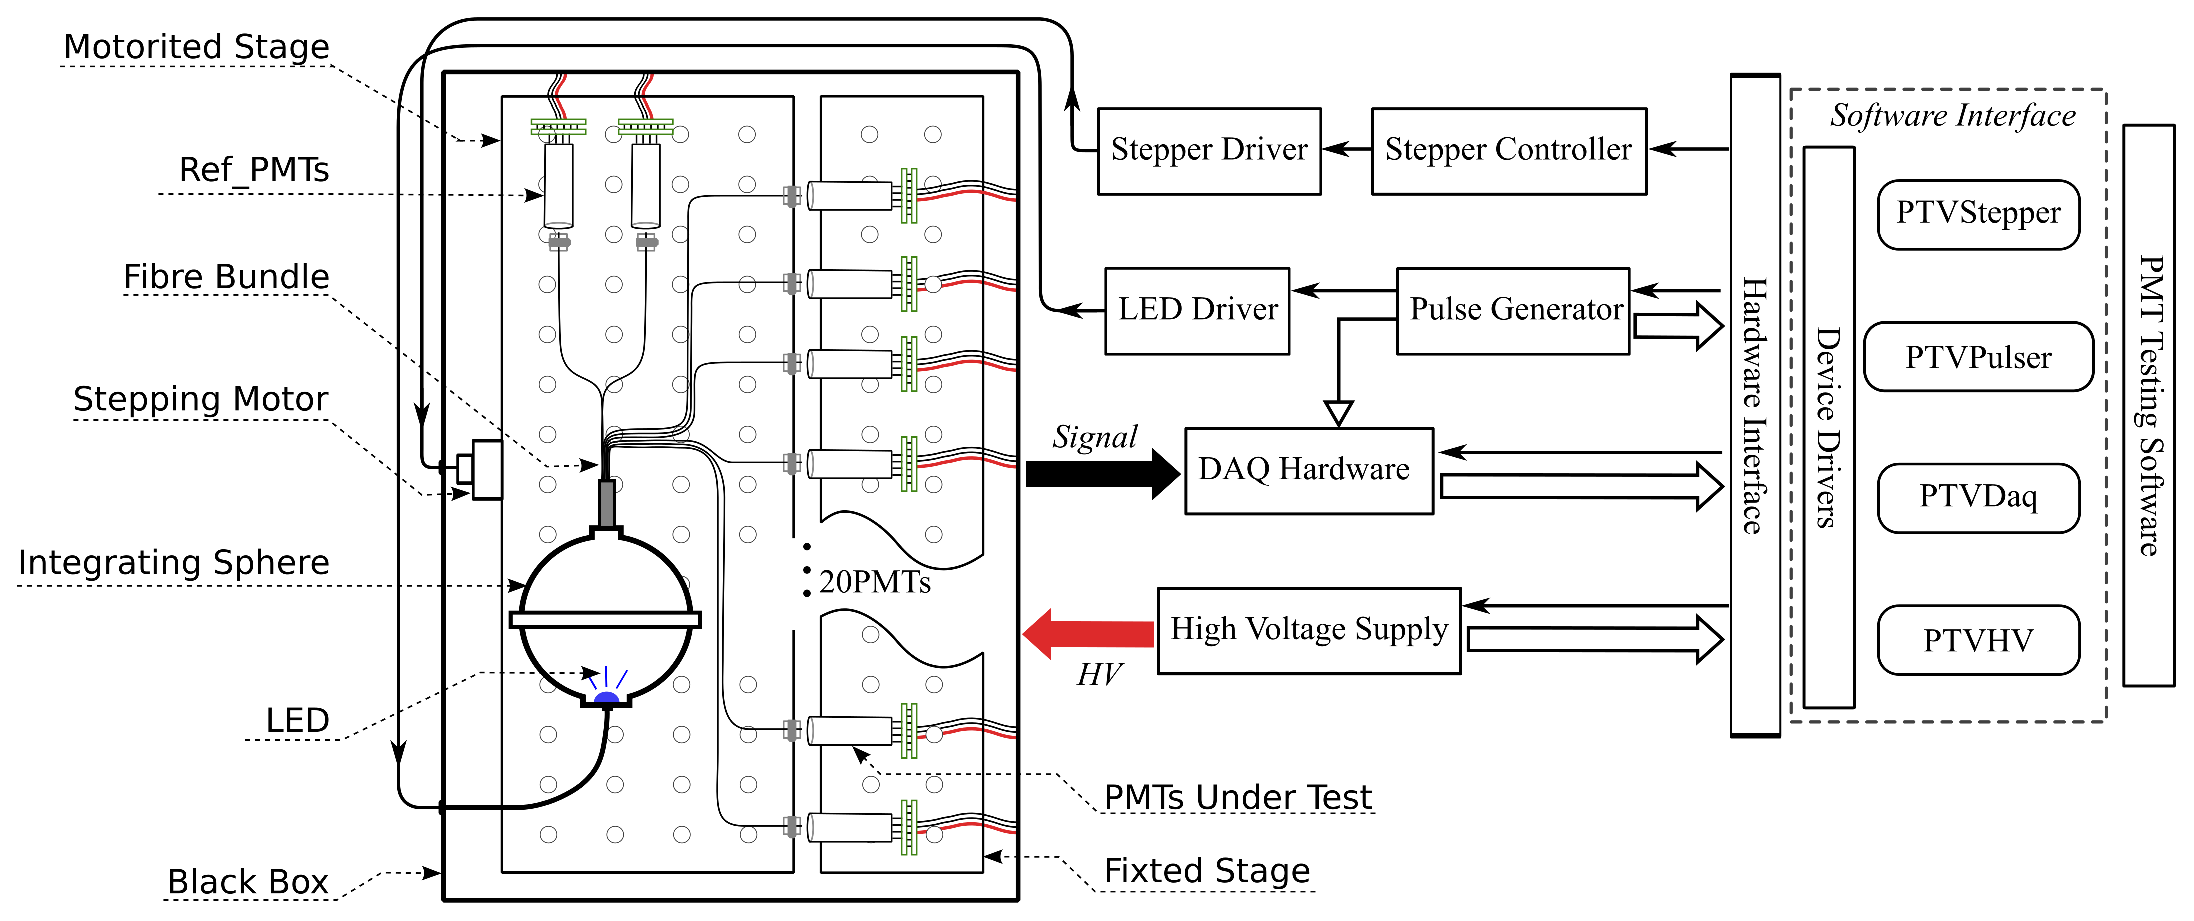
\includegraphics[width=140mm]{testbench_overview}
\caption{Schematic diagram of the PMT test bench system.\textit{PTVStepper}, \textit{PTVPulser}, \textit{PTVDaq} and \textit{PTVHV} are abstract classes which separate the testing software from the hardware implementation details.}
\label{fig:testbench_overveiw}
\end{figure*}

A schematic diagram of the final design is shown in Fig.\ref{fig:testbench_overveiw}.
The test bench is designed to test at least 20 R4443-Mod2 tubes in a single run.
Light flashes from a LED are distributed to each tube through an integrating sphere and a fibre bundle.
Tubes under test, including their bases, are mounted on a fixed stage, while the light source and its distribution system are mounted on a separate three-dimentional motorized stage.
%This allows position scanning of all tested tubes simultaneously.
Two additional PMTs are mounted in the corner of the motorized stage.
They will not be removed from their fixed positions during all test runs and thus are used as references to monitor the stability of the light source as well as the performance of the whole system.
Both stages are housed in a large light-tight box made of aluminium alloy, with the dimension of $176cm\times100cm\times78cm$.
The box is painted black inside and out and can be opened from the top plate for PMT mounting.
All other devices are located outside the light-tight box.
Cables are led out through various light-tight cable feedthroughs left in the side-plate of the box.
The test bench is sitted in a cleanroom of class 100000, the temperature of which is controlled around 22\textpm2\textcelsius~all the time.

In the following, each key component of the test bench will be described in detail.
\subsection{Motorized and Fixed Stages}
\label{sec:stages}

The motorized and fixed stages are the main body of the test bench.
They are arranged face to face with each other and are both covered with an optical breadboard of an area $1560mm\times250mm$, as shown in Fig.\ref{fig:stages}.
All other objects inside the light-tight box will be mounted on the top of them.
In particular, a specific fixture for R4443-Mod2 is designed that allows precise positioning of the tube with an accuracy of \textpm\SI{0.5}{\milli\meter}
The optical breadboards are made of \SI{2.5}{cm} thick stainless steel, which provides substantial resistance to deformation in this application.
The grid pattern of tapped holes on the surface facilitate mounting/unmounting operations, which not only increase efficiency but also provide extra flexibility in the configuration of the test system.

\begin{figure}[h!]
 \centering
 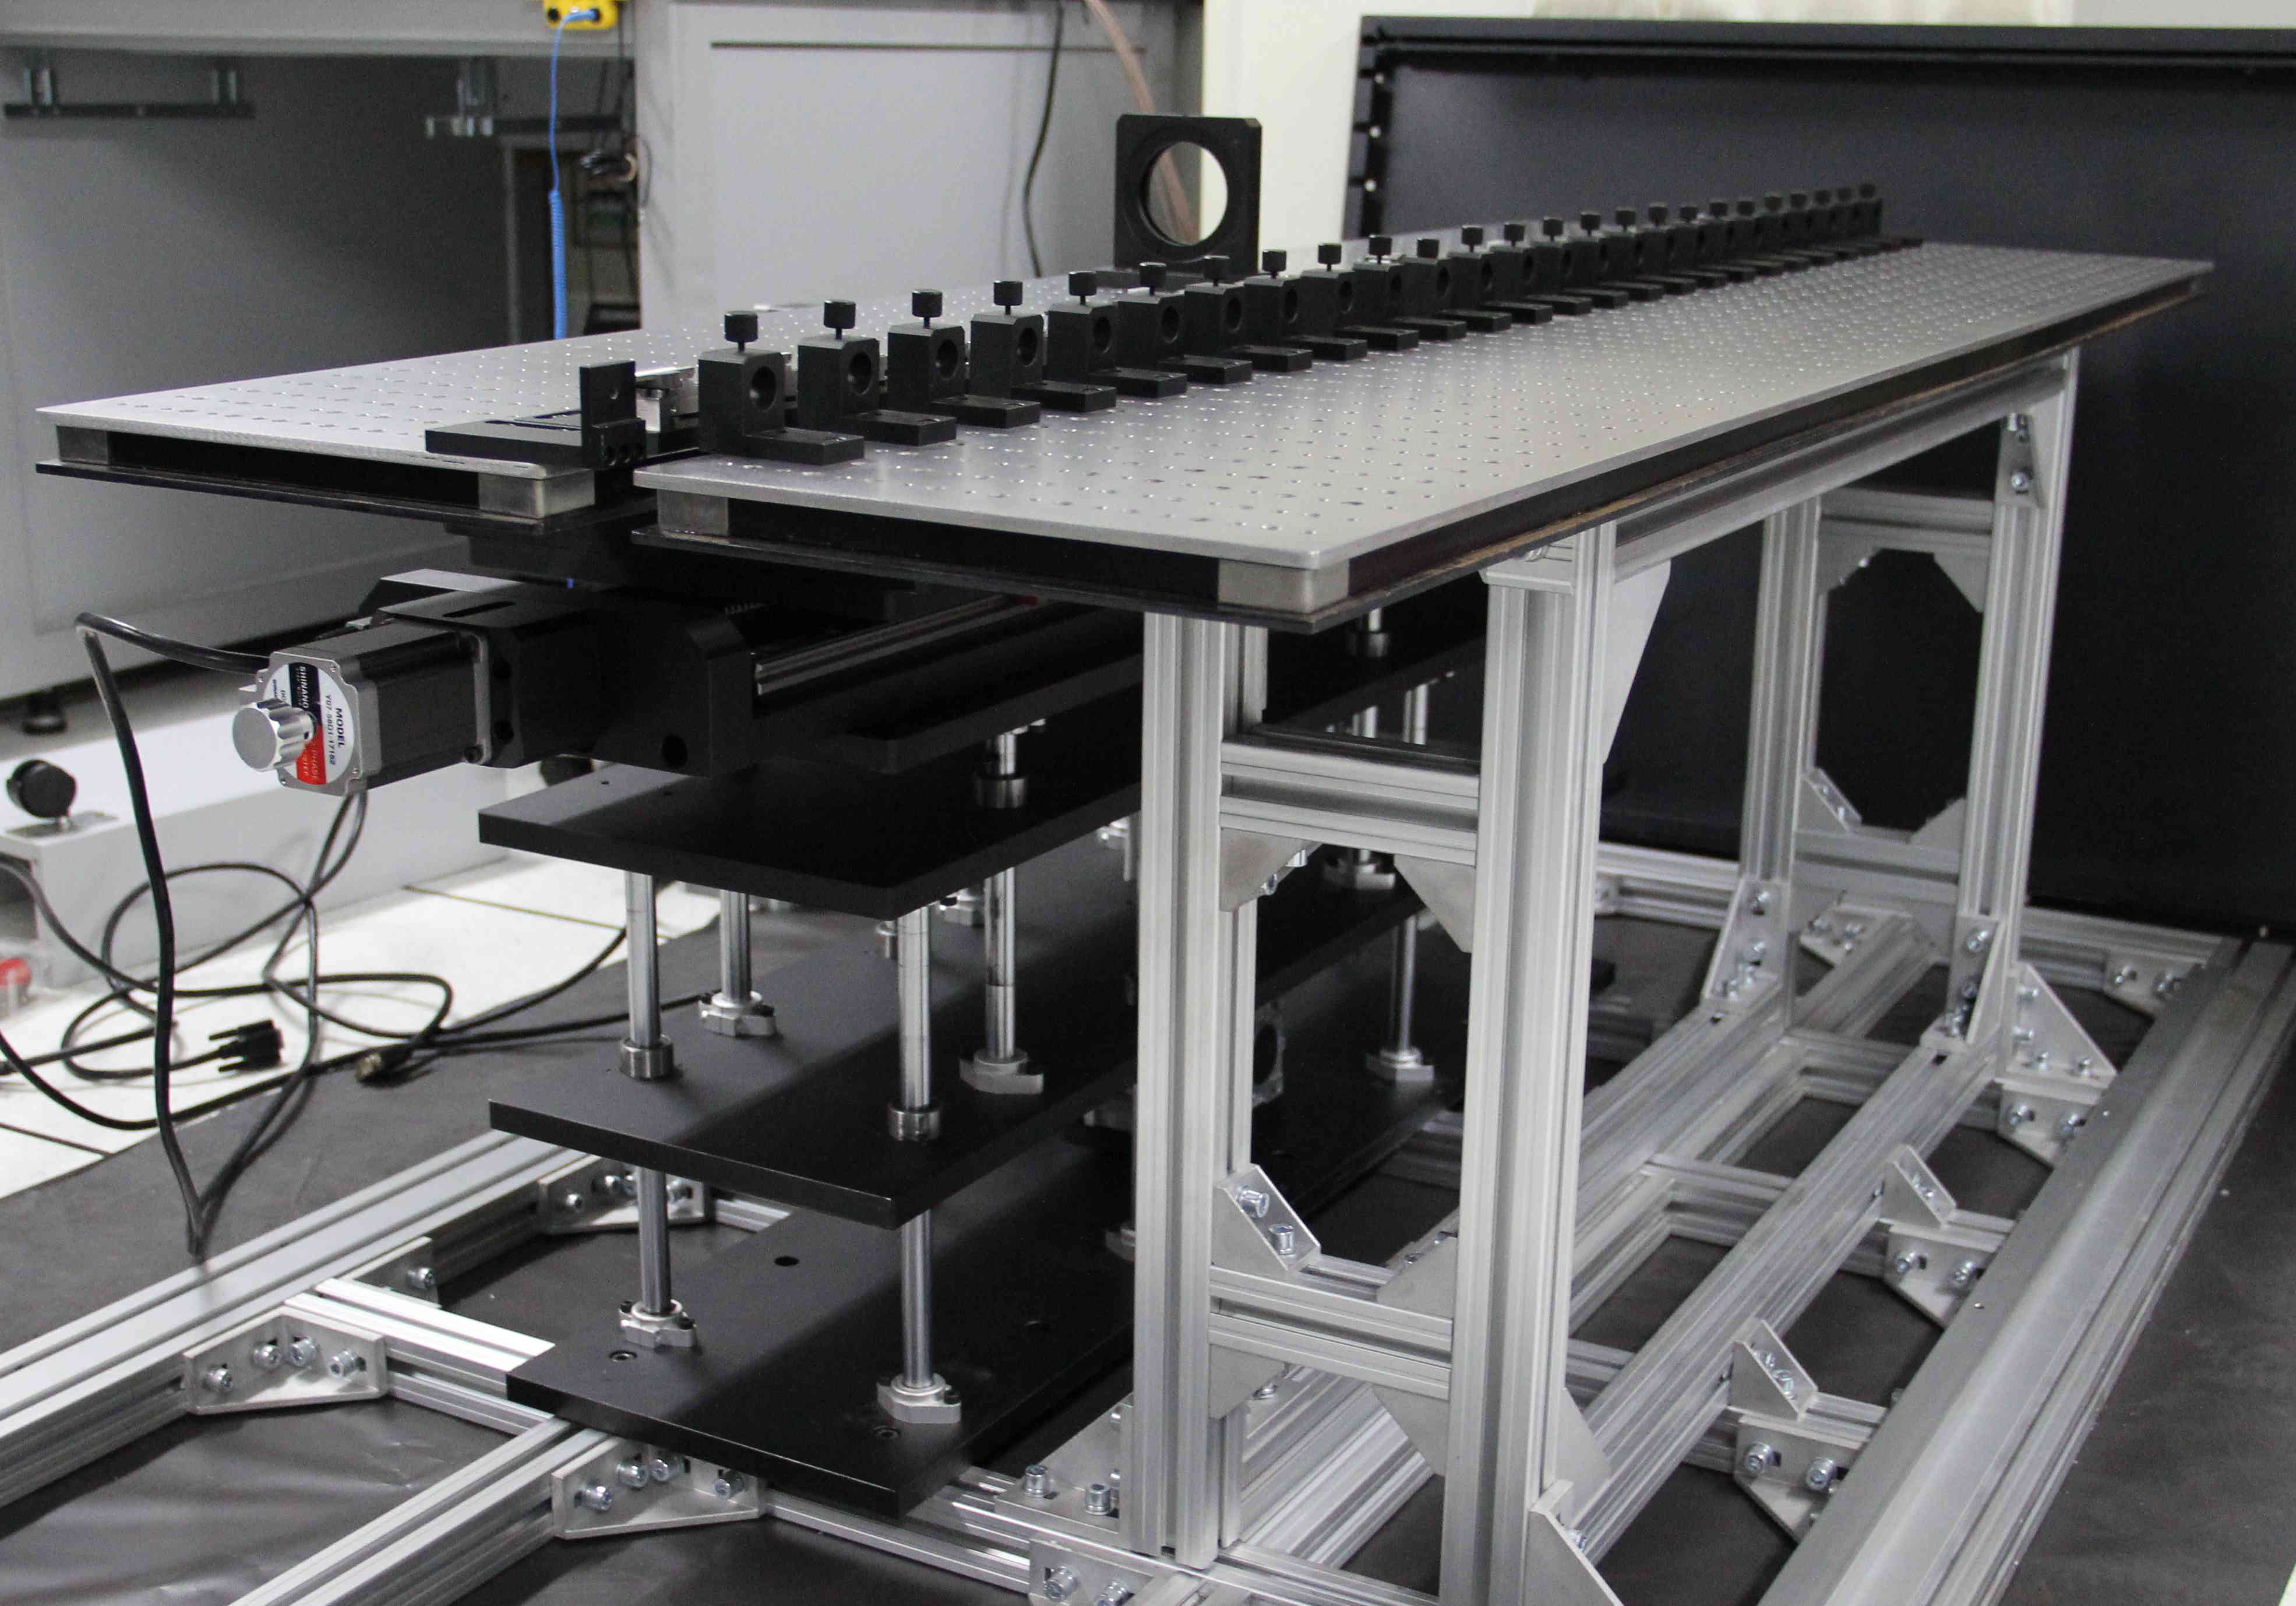
\includegraphics[width=90mm]{stage1_crop}
\caption{Motorized and fixed stages before assembly.}
\label{fig:stages}
\end{figure} 

Although not a primary concern in DAMPE PSD, the cathode uniformity of PMT is a critical characteristic in some applications, such as where bundled scintillating fibres or wavelenght shifting fibres are coupled to PMT and where multi-anode PMT is utilized for readout.
It's decided from the very beginning that position scanning capability should be added to the test bench.
The three-dimensional motorized stage is designed for this purpose.
%It will hold optical fibres, thus allowing scanning of the tubes fixed on the fixed stage.
The stage is driven by three stepping motors with a step size of \SI{1.56}{\micro\meter}.
The travel range in the horizontal direction and vertical direction is \SI{60}{\milli\meter} and \SI{70}{\milli\meter} respectively.
Thus the maximum scanning area is $60mm\times60mm$, which covers the size of the majority of PMTs and multi-anode PMTs.
The third direction with a travel range of $15mm$ is added to control the gap between the fibre and the tube's cathode surface.
This may be useful when extra space is needed for unmounting tubes without disturbing the optical fibres. 
The load capacity of the motorized stage is \SI{30}{\kilo\gram}.
All stepping motors are controlled by a single motion controller MPC07SP from Leetro.
MPC07SP can control up to 4 axises simultaneously and possesses a PCI interface for remote control and automation.

\subsection{Light Source and Distribution}
\label{sec:light_source}

A high-power blue LED(\SI{3}{\watt}, \SIrange{465}{485}{\nano\meter},  from Z-light~\cite{zlight}) is apdopted as the light source for the test bench.
This product has been used before in the monitoring and calibration system of Neutron Wall Detector at IMP, CAS~\cite{yuyuhong_led}. 
A \SI{5}{\centi\meter} diameter integrating sphere is used to convert the LED into a uniform light source.
The integrating sphere is coated interiorly with highly reflective material($\approx$\SI{98}{\percent} at \SI{400}{\nano\meter}) and has two ports of \SI{14}{\milli\meter} diameter.
To get better heat dissipation, the LED is fixed on a special designed base using thermally conductive silicone rubber.
The base is then coupled to the input port of integrating sphere, making the whole sphere as the LED's heat sink.

A bundle of 35 plastic clad silica(PCS) fibres is utilized to distribute light to each PMT under test.
The fibres are \SI{1.5}{\meter} long and have a \SI{400}{\micro\meter} diameter core and a \SI{550}{\micro\meter} diameter cladding.
The numerical aperture(NA) is 0.37.
The relatively large core and large NA make the fibre an efficient light extracter of integrating sphere output. 
The input end of the fibre bundle is coupled to the centre of the output port of integrating sphere using a three-dimensional fibre alignment stage.
On the other end, each fibre is fixed using a customized fibre holder which allows rough position adjustment individually.
Before testing, all used fibres are aligned to the centre of their corresponding PMT's input window with a precision of \SI{0.5}{\milli\meter}.  
For easier manipulation and to protect the fibres from mechanical stress, both ends of the fibre bundle are coated with customized stainless steel ferrules.

\begin{figure}[h!]
 \centering
 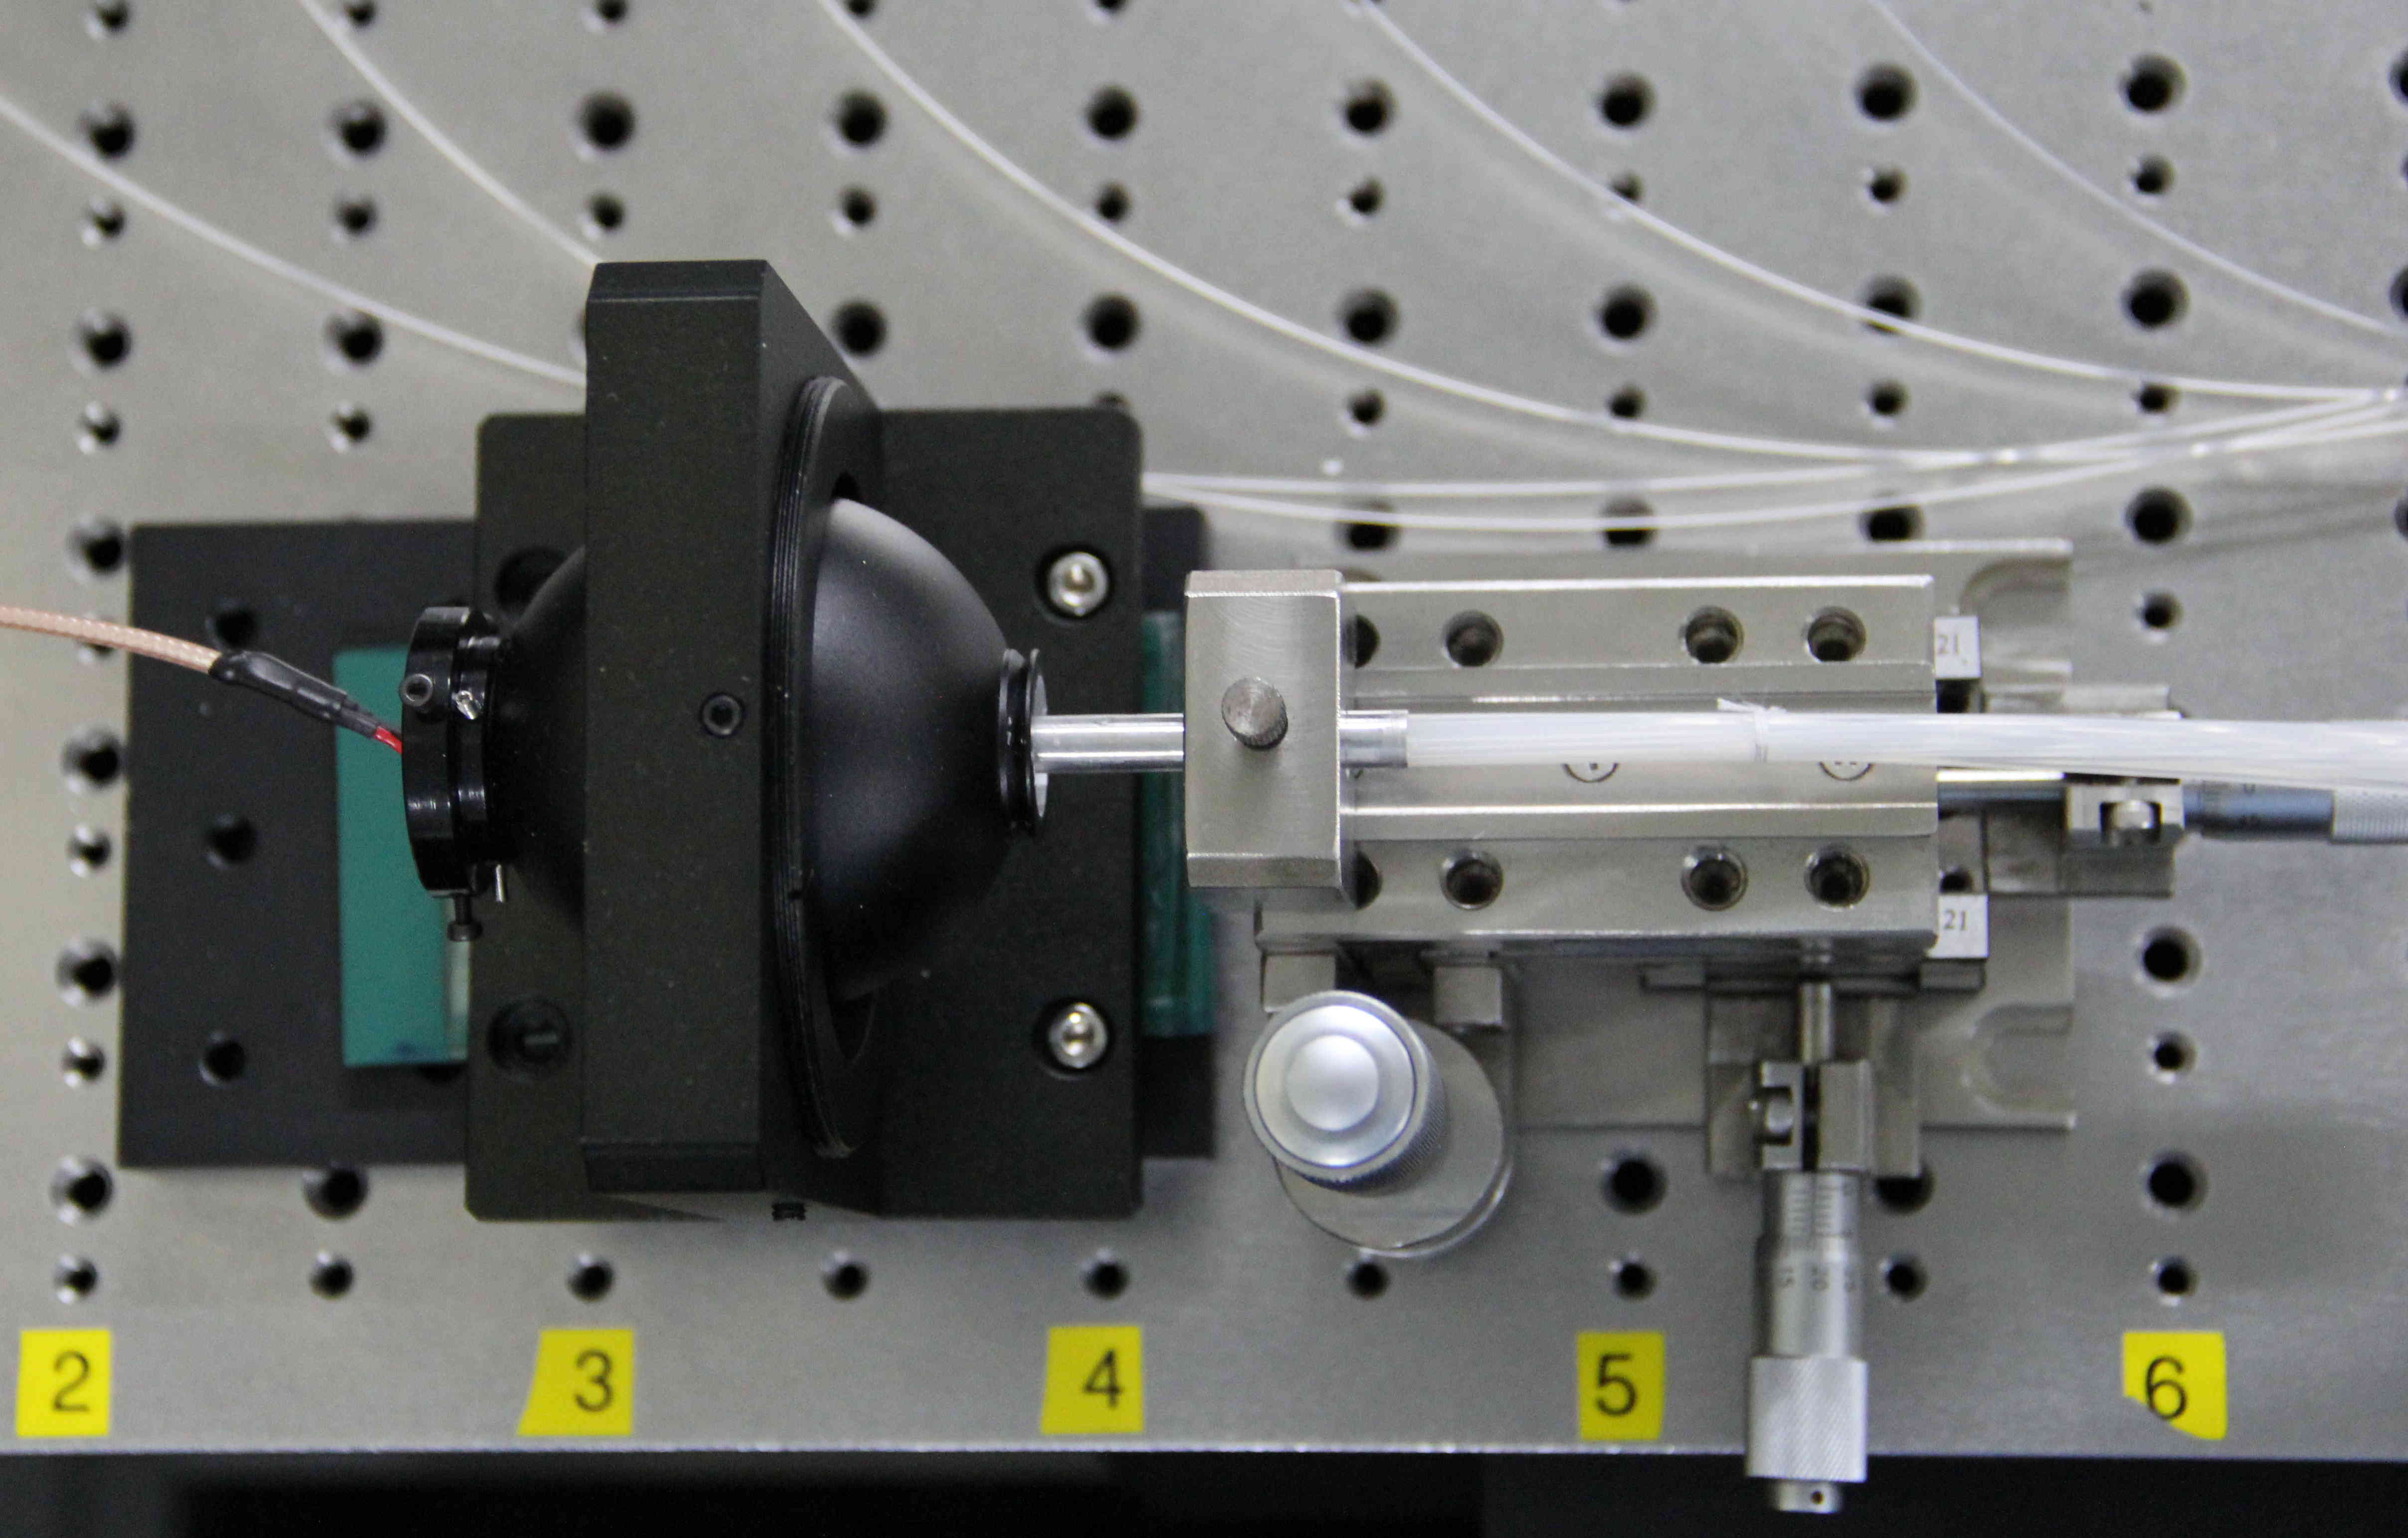
\includegraphics[width=90mm]{light_source1_crop}
\caption{Light source and its distribution system}
\label{fig:light_source}
\end{figure} 

\begin{figure}[h!]
 \centering
 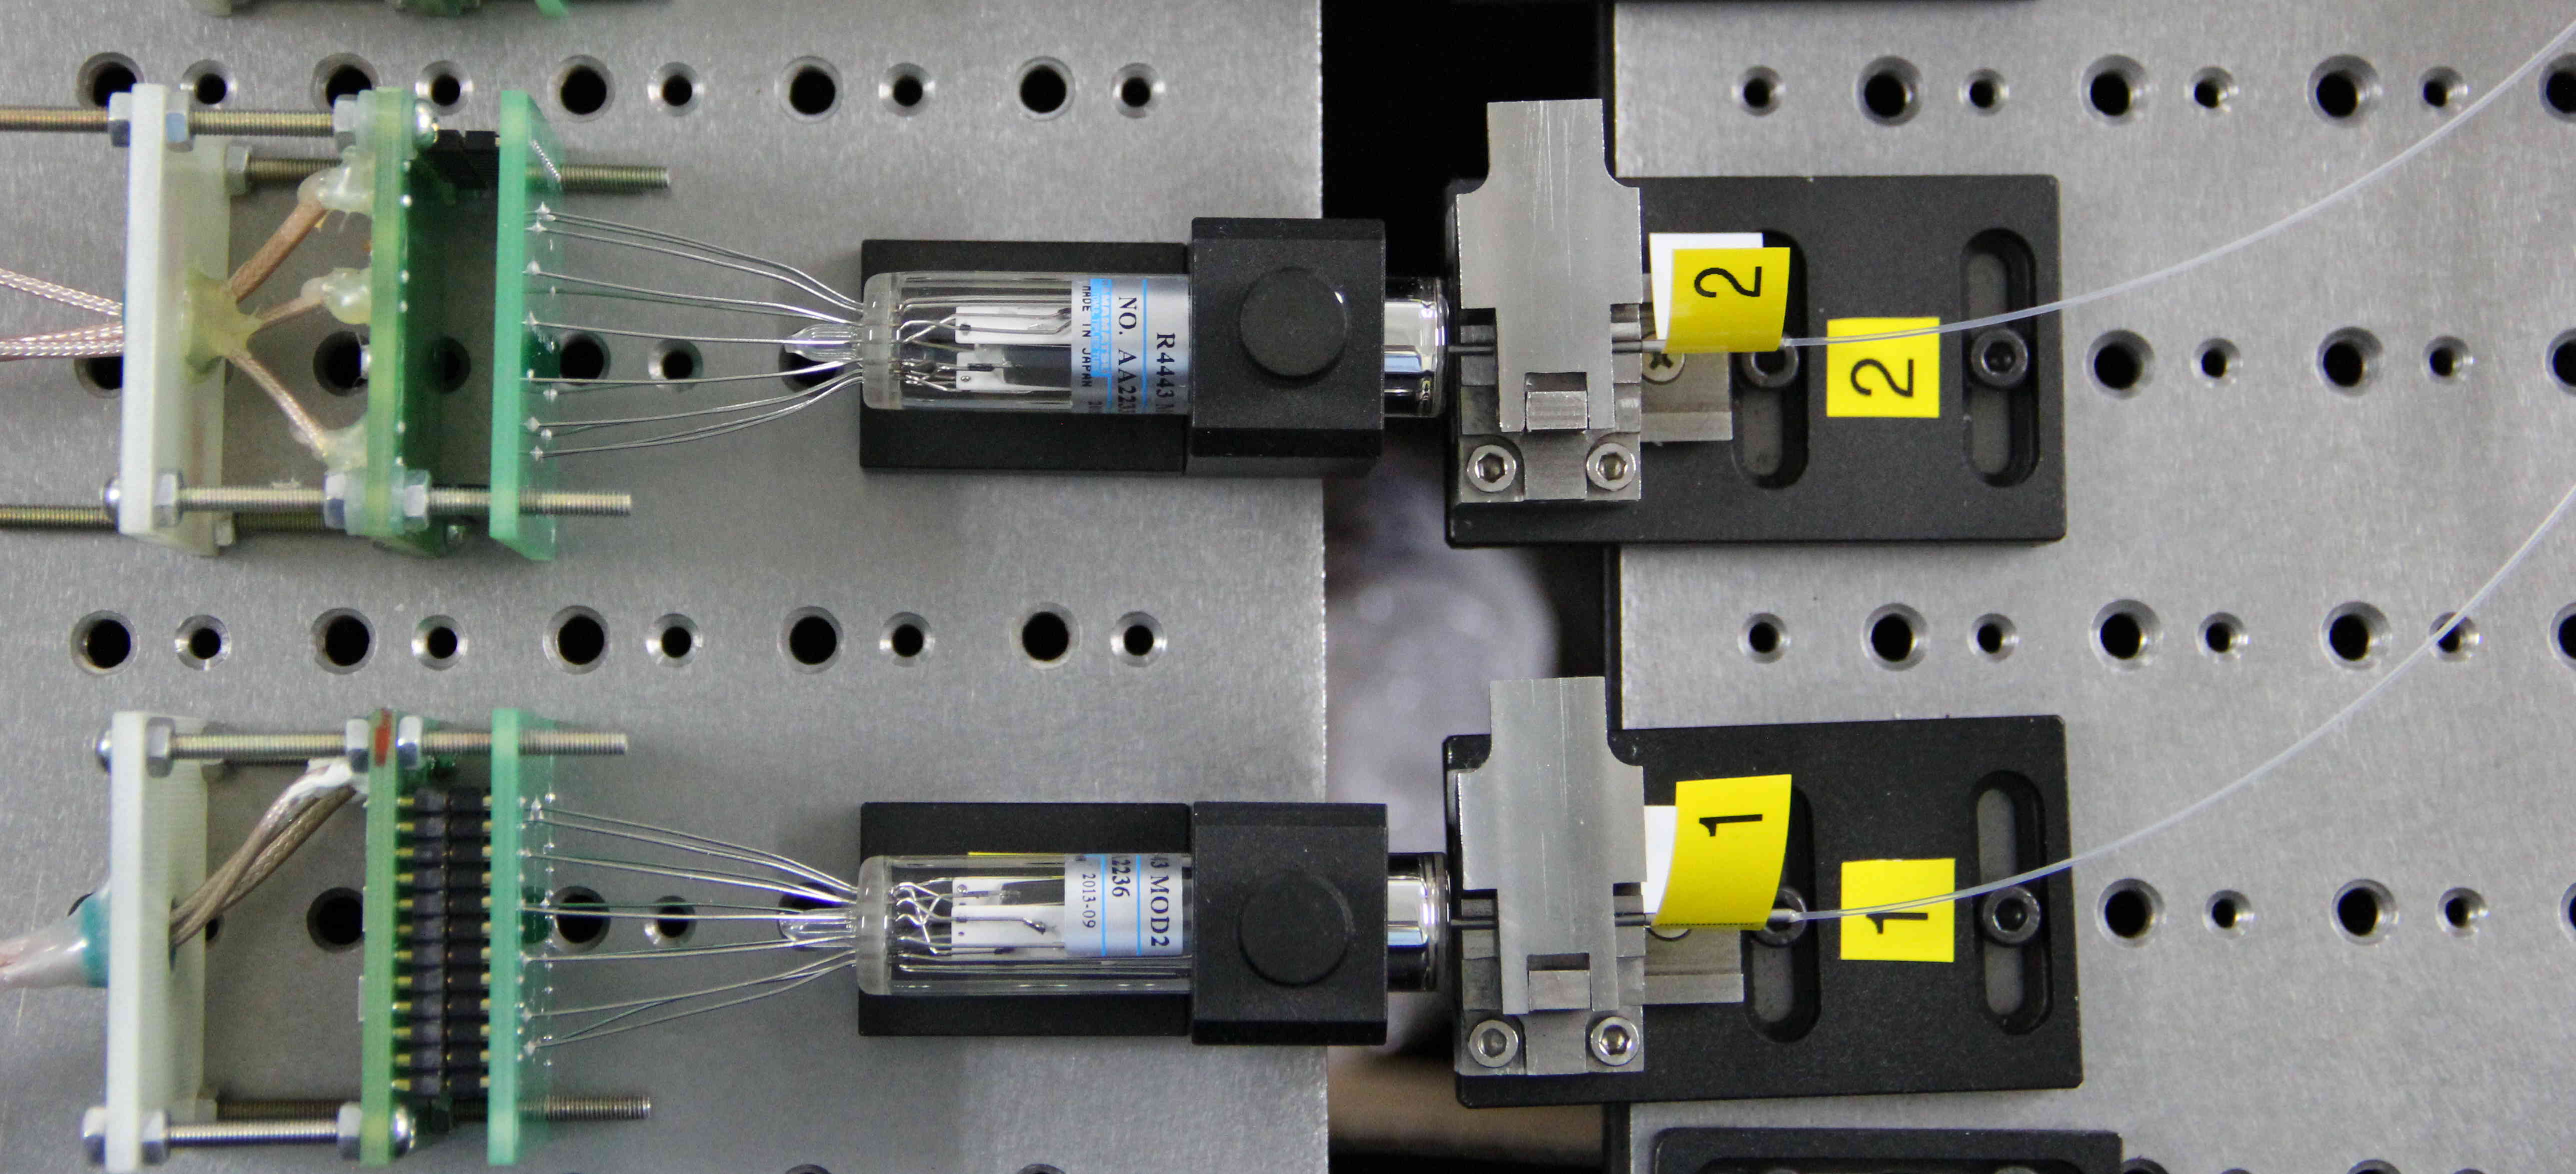
\includegraphics[width=90mm]{fixtures1_crop}
\caption{Special designed fixtures for tube and optical fibre are used}
\label{fig:fixture}
\end{figure}

\begin{figure*}[t]
 \centering
 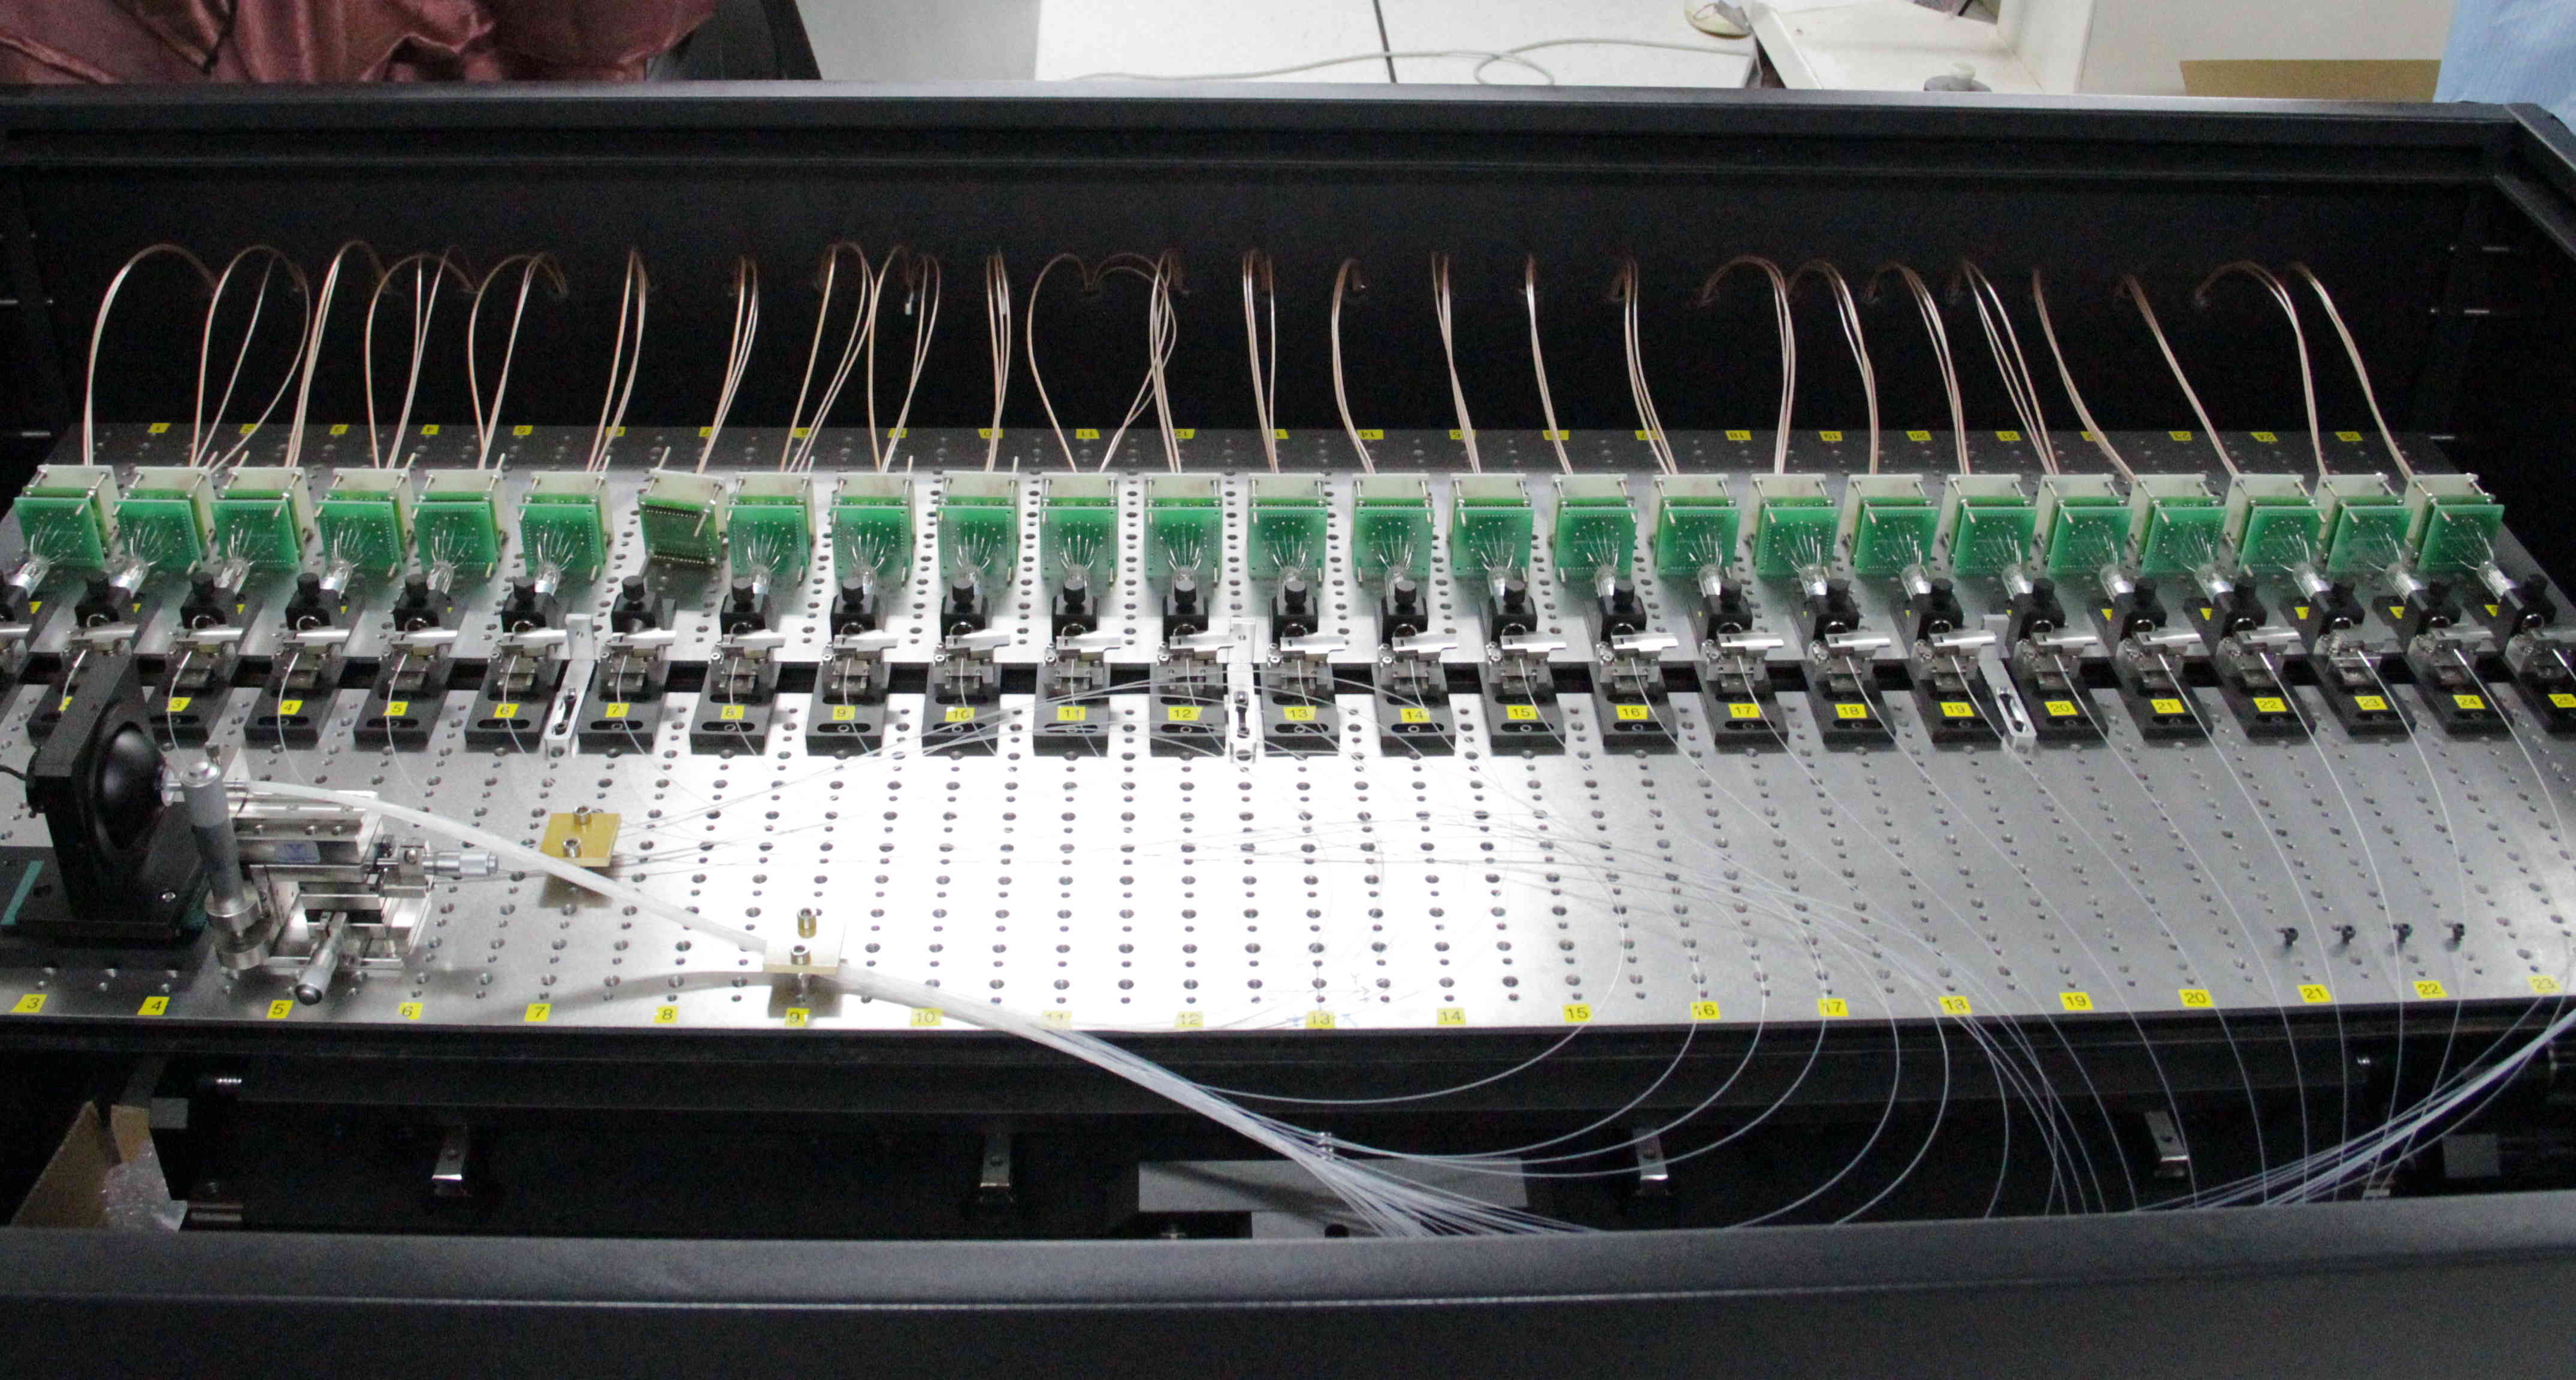
\includegraphics[width=140mm]{integration1_crop}
\caption{The integrated testbench,with tubes under test mounted.}
\label{fig:testbench_integrated}
\end{figure*}
  
An off the shelf hardware, Tektronix AFG3252 arbitrary/function generator, is adpoted as the LED driver.
As a commertial product, various interfaces for remote control are provided in AFG3252, making it suitable for automation.
All of the pulse parameters of AFG3252 can be adjusted in a wide range with high precison, as show in Table \ref{tab:afg3252}.
This is a critical feature for the PMT test of DAMPE PSD, as light intensities covering a large dynamic range are needed to measure the gain ratio between dynode 8 and dynode 5 at different voltages.
\begin{table}[h!]
\caption{Summary of AFG3252 Pulse Mode Characteristics}
\label{tab:afg3252}
 \begin{center}
 \begin{tabular}{lr}
 \multicolumn{2}{l}{Summary of AFG3252 pulse mode characteristics}\\ \hline
 Frequecny & up to \SI{120}{\MHz} \\
 Amplitude & max \SI{5}{\volt} \\
 Pulse width & min \SI{4}{\nano\second} \\
             & resolution \SI{10}{\pico\second} \\
 Leading edge & \SI{2.5}{\nano\second} to 0.625*pusle period \\
 Trailing edge & \SI{2.5}{\nano\second} to 0.625*pusle period \\
 Jitter(typical) & \SI{100}{\pico\second} \\
 Interface     & GPIB, LAN, USB
 \end{tabular}
 \end{center}
\end{table} 
AFG3252 has two independent analog outputs which can be synchronized together.
Thus it can output a trigger signal to DAQ at the same time it driving the LED. 
Although not designed to be a dedicated LED driver, the stability of AFG3252 is quite satifactory, see Sec.\ref{sec:longterm_stability}.
One limitation of AFG3252 as a LED driver is that it has a limited leading edge of \SI{2.5}{ns}.
This makes it not suitable for timing-related characterizations, where ultra-short(down to hundreds of \si{\pico\second} magnitude) light pulse is preferred.
In this casse, a dedicated LED driver of special design(commertial or home-made)may be used instead.
But AFG3252 can still be used as a trigger generator to control both the LED driver and DAQ.

\subsection{Electronics}
\label{sec:electronics}

To get more realistic results, electronics for PSD ground test is utilitized for the PMT test.
It consists of a front end electronics(FEE) box and a data acquisition(DAQ) board.
Both of them are standalone devices powered by a standalone DC power.
The FEE is based on the same design as the flight model of PSD, except that it uses commertial grade components instead.

Signals from R4443-Mod2 are connected to the FEE box directly and undergo charge integration and pusle shaping there.
Trigger signal from AFG3252 is connected to the DAQ board, which then dispatch the trigger to the FEE box.
Upon recieving the trigger, FEE will hold and digitize the shaped signal and transmit the digits to the DAQ board for packaging.
The packaged data are finally readout by a computer through the USB port on the DAQ board.
Commands from computer are sent to the DAQ board through a RS232 serial port.
Both the USB and serial interface are controlled using the NI-VISA library.

\subsection{High Voltage Supply}
\label{sec:hv}

The high voltage to PMTs is provided by a CAEN A1535SP board housed in the CAEN mainframe SY1527LC. 
A1535SP houses 24 independent positive HV channels, with an output range from \SIrange{0}{3500}{\volt}.
Current and voltage protection are provided by the board, thus allowing protection of the PMT from accidental ambient light exposure when HV is on.
Both current and voltage values can be set and monitored through the Ethernet interface of SY1527LC using the dynamic library provided by CAEN.

SY1527LC is a universal power supply system with 16 slots.
If needed, A1535SP can be replaced by other boards with more appropriate parameters, while the control interface remains unchanged.
Due to its multi-user feature, this mainframe is also shared by several other devices in the cleanroom.

\subsection{Software}
\label{sec:software}

\begin{figure*}
\centering
 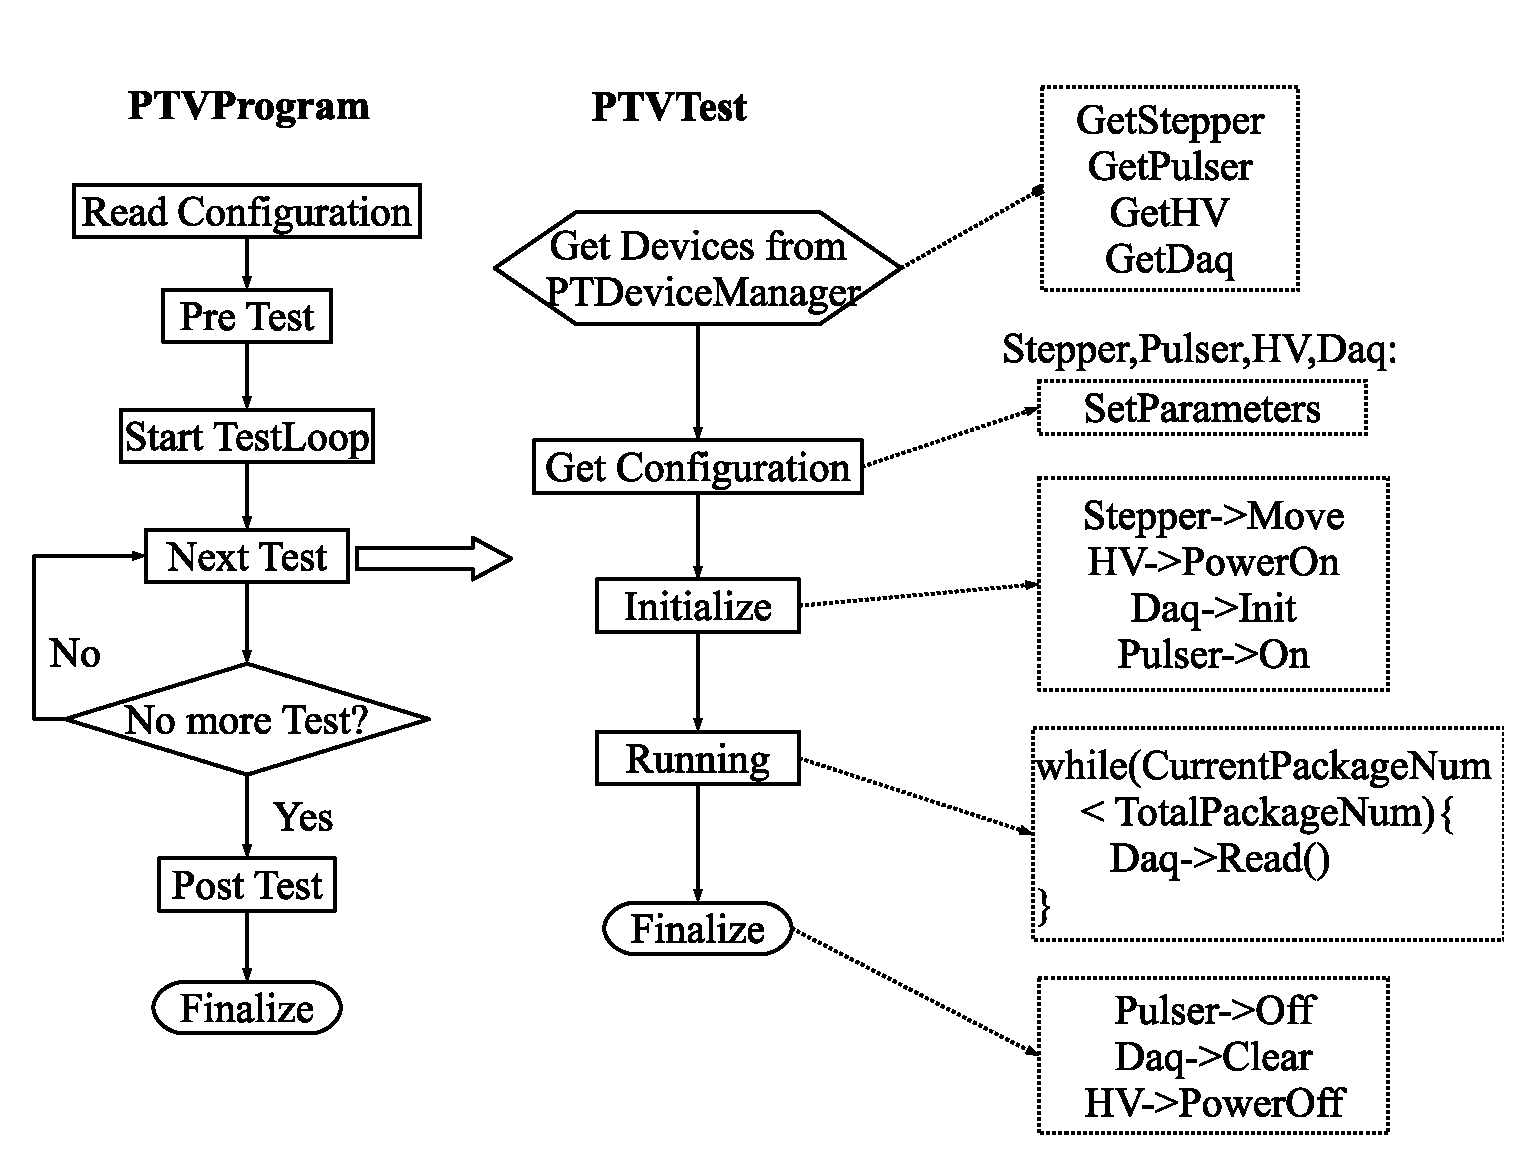
\includegraphics[width=140mm]{software_framework}
\caption{Software framework}
\label{fig:software_framework}
\end{figure*}

The software is developped under Windows and written in C++, which is an efficient language and well suited to the modular design of the test bench.
To facilitate maintainence and future upgrade, the software components are groupped into three hierarchies as follows:
\begin{enumerate}
 \item \textit{Device abstraction}, which not only serves as an interface to the underlying hardwares, but also handles the abstraction of different types of devices. 
 \item \textit{Framework libraries}, which defines a general testing procedure and provides utility classes for configuration and management.
 \item \textit{User inerface}, which provides command line based or graphical executables for user interaction. 
\end{enumerate}

Designed as a versatile equipment, different hardware modules may be used in the future.
For example, while the general-purpose VME or CAMAC platform may meet the demands of most of the use cases, some experiments may prefer to use project-specific DAQ hardware for testing, like the current case of DAMPE PSD.
%In another case, a laser light source with a ultra-short pulsing driver may be used for time-related characterization.
%For example, although project specific electronics are used in the PMT testing of DAMPE PSD, a DAQ system based on VME or CAMAC may meet the demands of most of the general-purpose characterizations.
Instead of developping a dedicated program each time a hardware interface changes, an abstraction of the devices is adoptted to separate the testing procedure from hardware implementation details. 
Abstract classes are defined for four frequently-used devices in PMT testing, i.e. motion controller, pulse generator, DAQ system and HV supplier, as shown in rounded boxes in Fig.\ref{fig:testbench_overveiw}.
Common operations of each type of device are extracted and encapsulated in the corresponding abstract class, which are the only interface to higher level software components.
Concrete classes inheritted from the same abstract class represent different devices of the same type.
Currently, device classes for MPC07SP motion controller, AFG3252 pulse generator, SY1527LC power supply system and PSD DAQ board for ground test are implemented.
DAQ device class for the CAMAC system based on CC-USB controller is also implemented and thoroughly tested.

Built upon the abstract device inerface, a general testing framework is defined.
As a first step, all used concrete device classes shall be registered in the singlton class \textit{PTDeviceManager}.
Devices are then retrieved from \textit{PTDeviceManager} during test, thus making the rest of the framework independent from specific hardwares.
The testing procedures are then grouped as shown in Fig.\ref{fig:software_framework}.
A \textit{PTVProgram} represents the measurement procedure for a specific characteristic of PMT, such as cathode uniformity, gain, dark count rate, and so on.
\textit{PTVTest} is a subunit of \textit{PTVProgram}, which encapsulates the real testing operations performed under a specific condition.
A typical implementation for \textit{PTVTest} using fake code is presented in the third column of Fig.\ref{fig:software_framework}.
Usually, a \textit{PTVProgram} consists of a series of \textit{PTVTest}s, which are invoked sequentially in a test loop.
For example, for cathode uniformity test, the stepping motor will move to a series of positions and the PMT response will be recorded by the DAQ system at each position.
Here, device operations performed at each position constitute a \textit{PTVTest} and tests at all positions constitute a \textit{PTVProgram}.
Additional actions may be added in the \textit{PreTest} method and \textit{PostTest} method of \textit{PTVProgram}, which will be invoked before and after the test loop repectively.
Typically, PMT warming shall be performed in \textit{PreTest} and analysis code shall be added in \textit{PostTest}.
\textit{PTVProgram}s of different testing objectives will finally be chained together to constitute a complete characterization of PMT.
Two concrete \textit{PTVProgram}s have been implemented for DAMPE-PSD PMT test.
One for pedestal testing and one for amplitude scan and voltage scan.

Based on the framework library, a light-weight user interface based on PDCurses~\cite{pdcurses} has been developped.
This program also incorporates status monitoring function, which is developped utilizing Phtread-win32 library~\cite{pthread_win32}.

A dedicated analysis program based on ROOT libraries is also developped for the DAMPE PSD project.
The program does not depends on the framework libraries described above.
The analysis results are inserted into a database for easy query.

\begin{comment}
\section{Characteristics of the test bench}
\label{sec:char_testbench}

\subsection{Spatial Uniformity of Integrating Sphere}
\label{sec:spatialuniformity_insph}

Before coupling to the fibre bundle,the spatial uniformity of the light source(LED + Integrating Sphere) is investigated. 
A single optical fibre of the same type as the fibre bundle in the test bench is utilitized.
One end of the fibre is fixed on a three-dimensional alignment stage and used to scan the output port horizontally and vertically in a \SI{1}{\milli\meter} step.
The other end is readout by a PMT of R4443-Mod2 and processed by the electronics of PSD groud test.
The LED is driven by a \SI{40}{\nano\second} width pulse of fixed amplitude at \SI{500}{\Hz}.
%The same LED signal is used during the scanning.

The result(Fig.~\ref{fig:uniformity_integratingsphere}) shows that the integrating sphere works as expected and the light intensity is almost the same(within \textpm0.5\%) over the entire surface of the output port.   


\begin{figure}[h!]
 \centering
 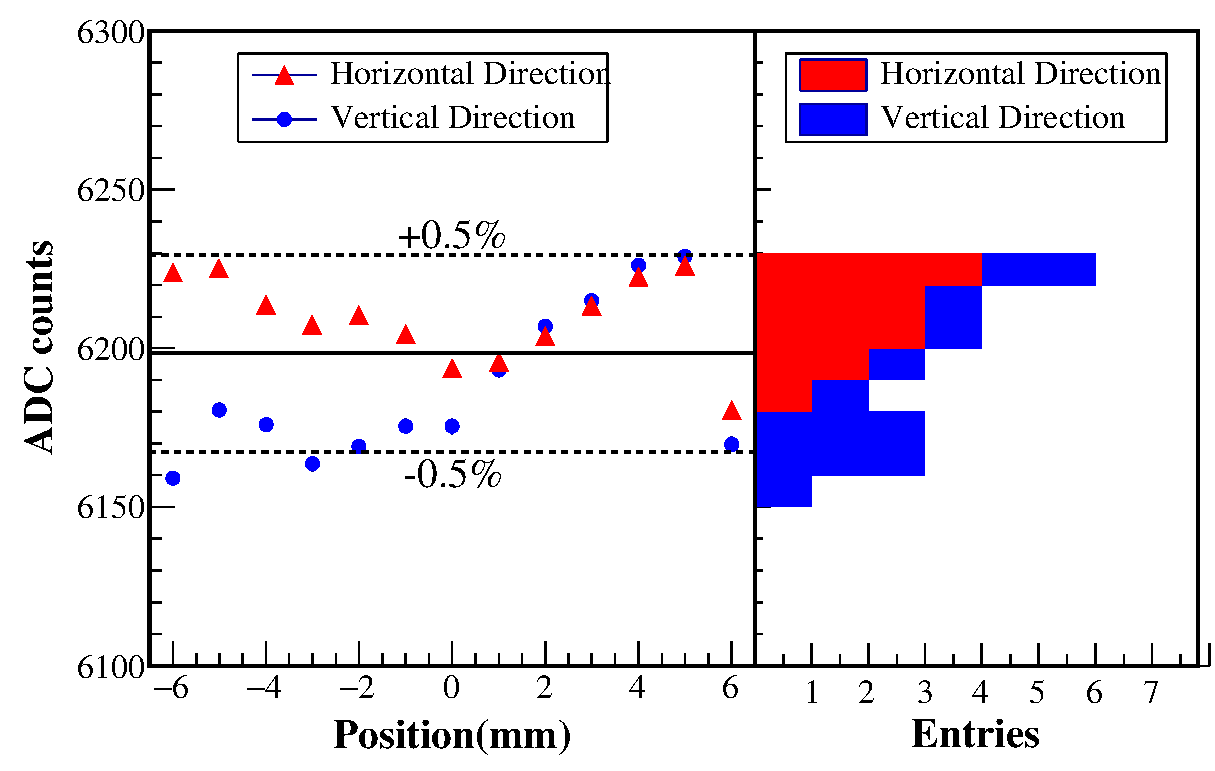
\includegraphics[width=90mm]{uniformity_integratingsphere}
\caption{Spatial uniformity of the integrating sphere.}
\label{fig:uniformity_integratingsphere}
\end{figure} 

\subsection{Transmission Uniformity of Fibre-bundle}
\label{sec:transuniformity_fibre}

The fibre bundle is then coupled to the integrating sphere and the output intensity of each fibre at the other end is tested.
As the test 

\subsection{Long-term Stability}
\label{sec:longterm_stability}

\end{comment}

\section{Application in the PMT testing for PSD of DAMPE}
\label{sec:application}


\subsection{Requirements of PSD}
\label{sec:psd_requirements}

\subsection{Testing Result of Relative Gain}
\label{sec:psd_gain}

\subsection{Testing Result of Dynode Ratio}
\label{sec:psd_dy58}

\subsection{Testing Result of Cathode Scan}
\label{sec:psd_cathodescan}

\subsection{Performance of the test bench during test}
\label{sec:performance}

%%%%%%%%%%%%%%%%  Conclustion   %%%%%%%%%%%%%%%%%%%%%%%
\section{Conclusions}
\label{sec:conclustions}

%%%%%%%%%%%%%%%% Acknowledgement %%%%%%%%%%%%%%%%%%%%%%%
\section*{Acknowledgement}

%%%%%%%%%%%%%%%%    Appendix     %%%%%%%%%%%%%%%%%%%%%%%
%% The Appendices part is started with the command \appendix;
%% appendix sections are then done as normal sections
\appendix
\section{}
\label{app:}

%%%%%%%%%%%%%%%%   Bibliography  %%%%%%%%%%%%%%%%%%%%%%%
%% bibliography style
\section*{References}
\bibliographystyle{elsarticle-num}

%% From BibTex file
\bibliography{mybib}

%% From hand-writing
\begin{comment}
%%\begin{thebibliography}{00}

%%\bibitem{CEBAF12}
%%V.D. Burkert,  \emph{arXiv:1203.2373v1 [nucl-ex]},  2012.

%%\bibitem{CLAS}
%%B.A. Mecking \emph{et al.},  Nucl. Ins. and Meth. in Phys. Research {\bf A503} (2003) 513

%%\end{thebibliography}
\end{comment}

\end{document}
\endinput